%\begin{tcolorbox}
%Teilt eure Klassendiagramme bitte auf und baut \textbf{kein} einzelnes riesiges Diagramm.
%Getter und Setter Methoden müssen hier nicht modelliert werden.
%Sie sollten aber der klassischen Namenskonvention folgen, um die Nutzung in Sequenzdiagrammen zu ermöglichen.
%\\\\
%Auf jedes Diagramm folgt eine Tabelle, in der die Aufgabe \textbf{jeder} Klasse beschrieben wird.
%\end{tcolorbox}


\section{Web}

\begin{figure}[h]
	\centering
	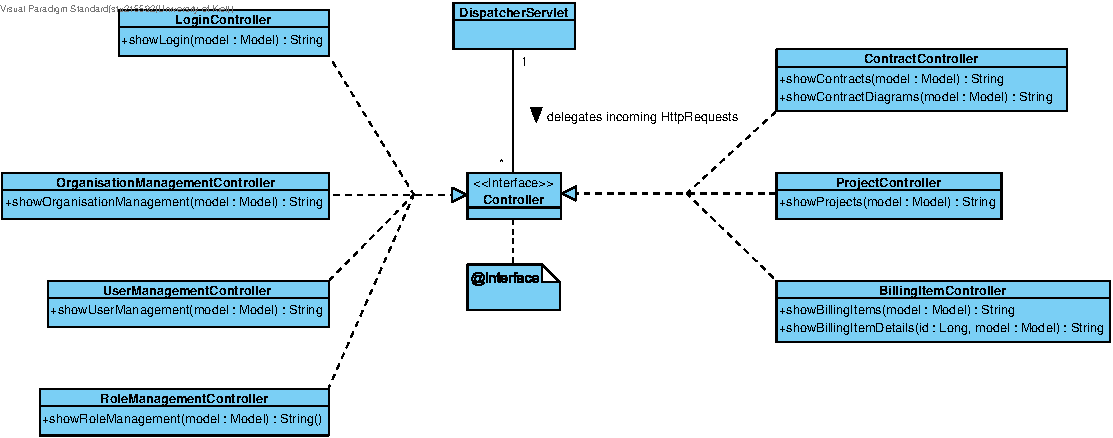
\includegraphics[width=\linewidth]{img/diagrams/Frontend Classes.pdf}
	\caption{Klassendiagramm - Frontend Web}
	\label{fig:klassendiagramm-web}
\end{figure}

\newpage

\noindent
Klassen, deren Name mit ''Controller'' aufhört, verarbeiten HTTP Requests zu bestimmten Pfaden.
Die zu verarbeitenden Pfade sind pro Gebiet in einem jeweiligen Controller gruppiert.
In der folgenden Tabelle werden für Controller unter ''Aufgabe'' die zu verarbeitenden Pfade sowie die Bedeutung der dazugehörigen Seite aufgeführt.
Die Identifikationsnummern oID (Organisation), diaID (Diagramm), pID (Projekt), cID (Vertrag) und bID (Leistungsposition) sind in manche Pfade direkt integriert.\\

\begin{longtable}[h]{p{5.3cm} p{8.7cm}}
	\caption{Klassenbeschreibung - Frontend Web}
	\label{table:klassenbeschreibung-web}
	\endlastfoot
	\multicolumn{2}{r}{{Weitergeführt auf der folgenden Seite}} \\
	\endfoot
	\endhead
	\rowcolor[HTML]{C0C0C0} 
	\textbf{Klassenname} & \textbf{Aufgabe} \\
    
	DispatcherServlet & Teil des Spring Frameworks, leitet die HTTP Requests an den jeweils zuständigen Controller weiter \\
	
	\rowcolor[HTML]{E7E7E7} 
	LoginController & /login $\rightarrow$ Login-Seite \\
	
	OrganisationManagementController & /organisation\_overview $\rightarrow$ Management von Organisationen und deren OrgAdmins \\
	
	\rowcolor[HTML]{E7E7E7} 
	UserManagementController & /user\_overview $\rightarrow$ Management aller WebUser \newline\newline
	/organisation/\{oID\}/user\_overview $\rightarrow$ Management der WebUser einer Organisation \newline\newline
	/organisation/\{oID\}/add\_user $\rightarrow$ Hinzufügen eines WebUsers zu einer Organisation \newline\newline
	/role\_overview $\rightarrow$ Management aller Rollen \newline
	/organisation/\{oID\}/role\_overview $\rightarrow$ Management der Rollen einer Organisation \newline\newline
	/organisation/\{oID\}/add\_role $\rightarrow$ Hinzufügen einer Rolle zu einer Organisation \\
	
	ProjectController & /project\_overview $\rightarrow$ Zeigt alle Projekte an, für welche der WebUser die nötigen Berechtigungen hat \newline\newline
	/project/\{pID\}/show $\rightarrow$ Zeigt die Verträge des Projekts an, für welche der WebUser die nötigen Berechtigungen hat \\
	
	\rowcolor[HTML]{E7E7E7} 
	ContractController & /contract\_overview $\rightarrow$ Zeigt alle Verträge an, für welche der WebUser die nötigen Berechtigungen hat \newline\newline
	/project/\{pID\}/contract/\{cID\}/show $\rightarrow$ Zeigt die Leistungspositionen des Vertrags an, für welche der WebUser die nötigen Berechtigungen hat \newline\newline
	/diagram\_overview $\rightarrow$ Zeigt alle Diagramme an, für welche der WebUser die nötigen Berechtigungen hat \newline\newline
	/project/\{pID\}/contract/\{cID\}/create\_diagram $\rightarrow$ Erstellen eines Diagramms \newline\newline
	/project/\{pID\}/contract/\{cID\}/diagram/\{diaID\}/show $\rightarrow$ Zeigt das Diagramm im Detail an \\
	
	BillingItemController & /billing\_item\_overwiew $\rightarrow$ Zeigt alle Leistungspositionen an, für welche der WebUser die nötigen Berechtigungen hat \newline\newline
	/project/\{pID\}/contract/\{cID\}/billing\_item/\{bID\}/show $\rightarrow$ Zeigt Details zur Leistungsposition an
\end{longtable}

\clearpage


\section{Backend}

\begin{figure}[h]
	\centering
	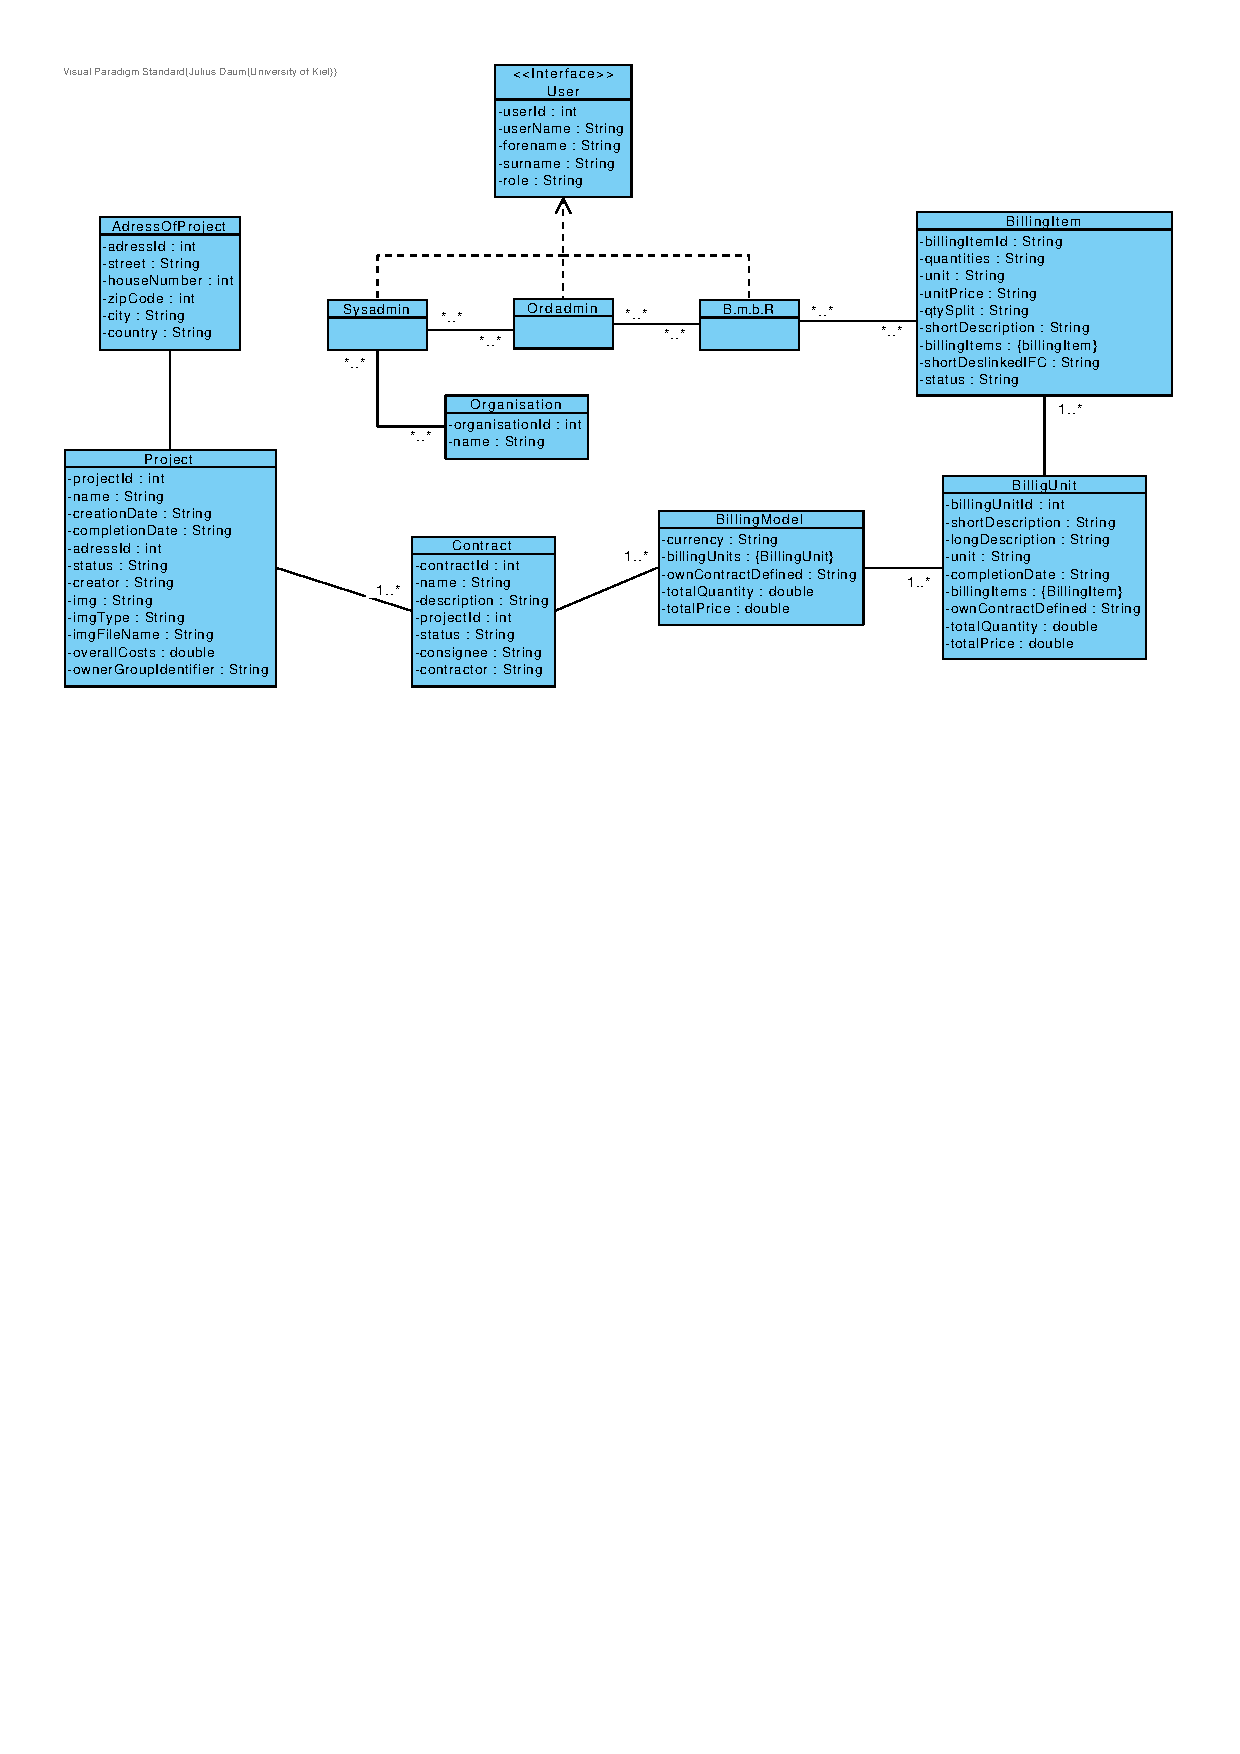
\includegraphics[width=\linewidth]{img/diagrams/class-diagram-backend.pdf}
	\caption{Klassendiagramm - Backend}
	\label{fig:klassendiagramm-backend}
\end{figure}

\newpage

\noindent
Dieses Klassendiagramm enthält die Entitäten der Datenbank, jede Klasse entspricht einer Entität. \\
Jede wichtige Klasse hat eine Assoziation zur Rolle, um die Authentifizierung zu gewährleisten. \\
Da SysAdmin und OrgAdmin überall einsehen können, assoziiert somit jede Klasse min. 2 Rollen.

\begin{longtable}[h]{p{5.3cm} p{8.7cm}}
	\caption{Klassenbeschreibung - Backend}
	\label{table:klassenbeschreibung-backend}
	\endlastfoot
	\multicolumn{2}{r}{{Weitergeführt auf der folgenden Seite}} \\
	\endfoot
	\endhead
	\rowcolor[HTML]{C0C0C0} 
	\textbf{Klassenname} & \textbf{Aufgabe} \\
    
	Address & Die Adresse des Projektes. \\
	
	\rowcolor[HTML]{E7E7E7} 
	BillingItem & Die Leistungspositionen eines Vertrages. \\
	
	BillingUnit & Eine Gruppierung von Leistungspositionen. \\
	
	\rowcolor[HTML]{E7E7E7} 
	Contract & Ein Vertrag, welcher zwischen zwei Parteien geschlossen wird. \\
	
	Organisation & Eine Gruppierung von Usern. \\
	
	\rowcolor[HTML]{E7E7E7} 
	Project & Ein Projekt min. einer Organisation, welches mehrere Verträge enhalten kann. \\
	
	Role & Nutzerrollen mit verschiedenen Rechten. Verwaltbar vom OrgAdmin. \\

	\rowcolor[HTML]{E7E7E7}
	User & Mitarbeiter min. einer Organisation.
\end{longtable}


\clearpage

\section{App}

\begin{figure}[h]
	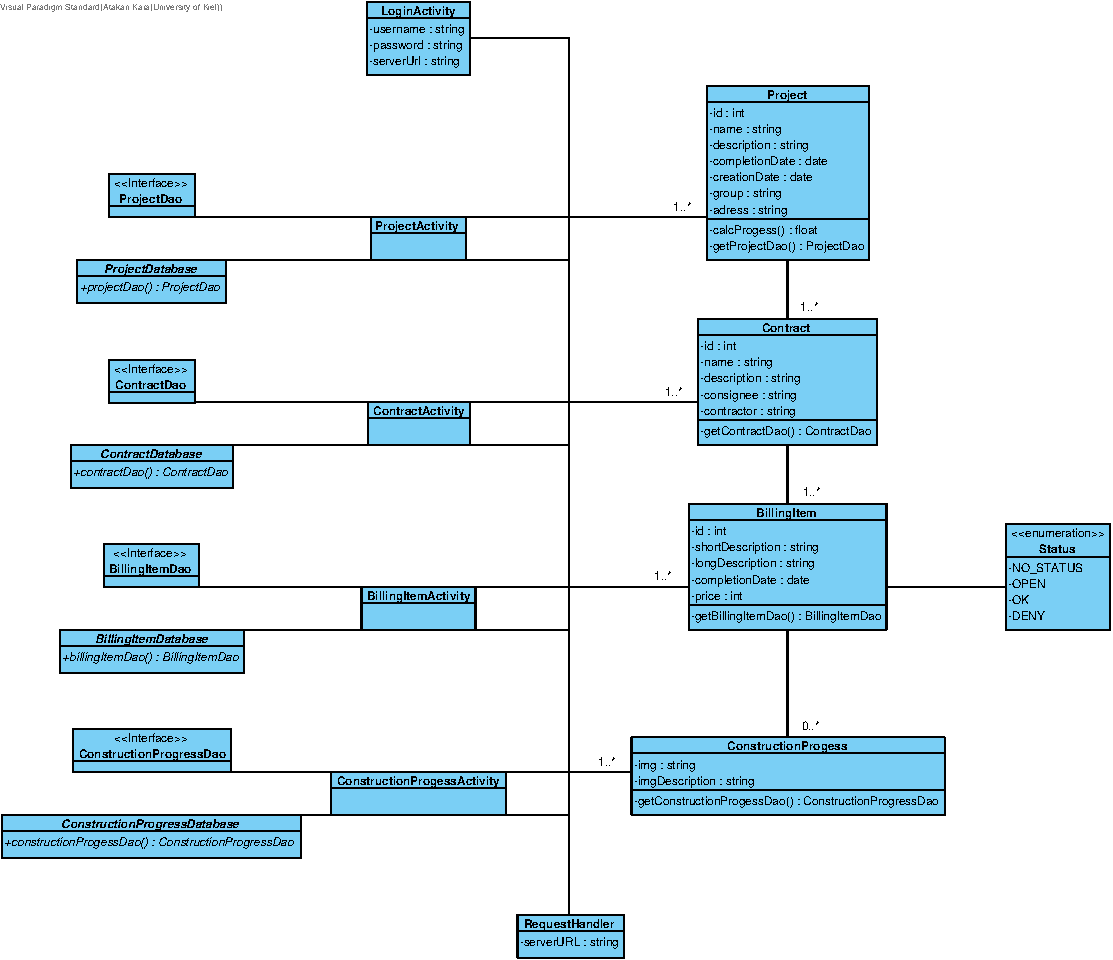
\includegraphics[width=16cm]{img/diagrams/Classdiagram-App.pdf}
	\caption{Klassendiagramm - App}
	\label{fig:klassendiagramm-a}
\end{figure}

\begin{table}[h]
	\centering
	\begin{tabularx}{\textwidth}{X X}
		\rowcolor[HTML]{C0C0C0} 
		\textbf{Klassenname} & \textbf{Aufgabe} \\
		Project & Bauplan eines Projektes mit den jeweiligen Attributen.\\
		\rowcolor[HTML]{E7E7E7} 
		Contract & Bauplan eines Vertrages mit den jeweiligen Attributen. \\
		BillingItem & Bauplan einer Leistungsposition mit den jeweiligen Attributen. \\
		\rowcolor[HTML]{E7E7E7} 
		ConstructionProgress & Bauplan einer Baufortschritts-Klasse mit den jeweiligen Attributen. \\
		LoginActivity & Verwaltung des Login-Bildschirms. \\
		\rowcolor[HTML]{E7E7E7} 
		ProjectActivity & Verwaltung des Projekt-Bildschirms. \\
		ContractActivity & Verwaltung des Vertags-Bildschirms. \\
		\rowcolor[HTML]{E7E7E7} 
		BillingItem & Verwaltung des Leistungspositions-Bildschirms. \\
		ConstructionProgressActivity & Verwaltung des Baufortschritts-Bildschirms. \\
		\rowcolor[HTML]{E7E7E7} 
		RequestHandler & Verwaltung der Netzwerkanfragen aller Klassen. \\
		ProjectDao & Datenzugriffsobjekt mit Anfragen zur Interaktion mit der Projektdatenbank. \\
		\rowcolor[HTML]{E7E7E7} 
		ProjectDatabase & Room-Datenbank für Projekte. \\
		ContractDao & Datenzugriffsobjekt mit Anfragen zur Interaktion mit der Vertragsdatenbank. \\
		\rowcolor[HTML]{E7E7E7} 
		ContractDatabase & Room-Datenbank für Verträge. \\
		BillingItemDao & Datenzugriffsobjekt mit Anfragen zur Interaktion mit der Leistungspositionsdatenbank. \\
		\rowcolor[HTML]{E7E7E7} 
		BillingItemDatabase & Room-Datenbank für Leistungspositionen. \\
		ConstructionProgressDao & Datenzugriffsobjekt mit Anfragen zur Interaktion mit der Baufortschritsdatenbank. \\
		\rowcolor[HTML]{E7E7E7} 
		ConstructionProgressDatabase & Room-Datenbank für den Baufortschritt. \\
		Status & Enumeration des Typs Status.
	\end{tabularx}
	\caption{Klassenbeschreibung - App}
	\label{table:klassenbeschreibung-a}
\end{table}

\clearpage
